\chapter{Diseño del videojuego}

En este capítulo se describe el diseño general de \textit{NeuroForge}, abordando sus mecánicas principales, reglas de juego y los elementos que definen su experiencia estratégica. Se detallan el funcionamiento del sistema de juego, la interacción con el jugador, la ambientación y el público al que va dirigido.

% ─────────────────────────────────────────────────────────────────────────────
\section{Resumen del videojuego}
% ─────────────────────────────────────────────────────────────────────────────

\textit{NeuroForge} es un videojuego de estrategia por turnos para un jugador inspirado en el clásico \textit{Stratego}. Dos bandos se enfrentan en un tablero de $10 \times 10$ casillas: el jugador humano y un oponente controlado por la máquina. El objetivo es destruir el \textbf{núcleo de energía} rival o dejarlo sin movimientos posibles.

Cada bando despliega en secreto un conjunto de piezas de distintos rangos en las cuatro filas más cercanas a su borde del tablero. Las identidades permanecen ocultas para el rival hasta que dos piezas entran en combate, momento en el que ambas se revelan y se resuelve el enfrentamiento según su rango.

En cada turno, el jugador puede realizar una única acción:, mover una pieza a una casilla adyacente vacía, o moverla a una casilla ocupada por una pieza enemiga para iniciar un combate. Existe una excepción, los \textbf{exploradores}, que pueden desplazarse varias casillas en línea recta en un mismo turno. El combate se resuelve de la siguiente forma:

\begin{itemize}
	\item La pieza de mayor rango vence y ocupa la casilla de la derrotada.
	\item Si ambas piezas tienen el mismo rango, ambas son eliminadas del tablero.
	\item Ciertas piezas tienen reglas especiales que se detallan más adelante.
\end{itemize}

% ─────────────────────────────────────────────────────────────────────────────
\section{Mecánicas}
% ─────────────────────────────────────────────────────────────────────────────

Gran parte del atractivo de \textit{NeuroForge} reside en el desconocimiento mutuo de la identidad de las piezas rivales. Esto convierte la deducción y el engaño en elementos estratégicos centrales: el jugador debe inferir la disposición del enemigo a partir de su comportamiento, al tiempo que protege la información sobre sus propias piezas.

\subsection{Tablero}

El tablero es una cuadrícula de $10 \times 10$ casillas (Figura~\ref{fig:EsquemaTablero}). Las cuatro filas más próximas a cada borde constituyen el \textbf{área de despliegue} de cada jugador, donde se colocan las piezas al inicio de la partida. Las dos filas centrales permanecen despejadas al comienzo y son terreno neutral.

En el centro del tablero se encuentran \textbf{casillas intransitables}, dispuestas en dos zonas de $2 \times 2$. Ninguna pieza puede moverse a ellas, ocuparlas ni atravesarlas. Estos obstáculos dividen el tablero en dos mitades y condicionan las rutas de ataque y defensa, actuando como cuellos de botella que añaden profundidad táctica al posicionamiento.

\begin{figure}[h!]
	\centering
	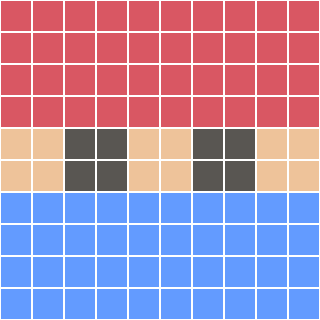
\includegraphics[width=0.32\linewidth]{../Imagenes/EsquemaTablero}
	\caption{Esquema del tablero}
	\label{fig:EsquemaTablero}
\end{figure}

\subsection{Colocación inicial}

Al inicio de cada partida, ambos bandos colocan sus piezas dentro de su respectiva área de despliegue con la distribución que consideren oportuna. No es posible colocar piezas fuera de dicha área antes de comenzar la partida. Una vez confirmada la colocación, la partida da comienzo y ningún jugador conoce la identidad de las piezas rivales.

La fase de despliegue tiene un peso estratégico considerable: una disposición bien planificada puede proteger las piezas clave, dificultar la deducción del rival y preparar aperturas ofensivas o defensivas para los primeros turnos.

\subsection{Piezas}

Las piezas se rigen por un sistema de rangos que determina el resultado de los combates: la pieza de mayor rango vence a la de menor rango. Cada tipo de pieza tiene una cantidad limitada por bando. Algunas piezas cuentan con propiedades especiales que modifican las reglas generales de movimiento o combate. A continuación se describen todos los tipos disponibles:

\begin{itemize}
	\item \textbf{Núcleo de energía (cantidad: 1):} La pieza más importante del bando. No puede moverse. Su destrucción supone la derrota inmediata de su propietario, y puede ser atacado por cualquier pieza enemiga capaz de moverse.
	
	\item \textbf{Torretas automáticas (cantidad: 6):} Estructuras defensivas inmóviles que no pueden atacar, pero destruyen automáticamente cualquier pieza que las ataque, independientemente de su rango. La única excepción son los \textbf{saboteadores}, que son los únicos capaces de destruirlas.
	
	\item \textbf{Máquina de guerra (cantidad: 1, rango 10):} La unidad de combate más poderosa. Vence a cualquier pieza por rango, salvo al \textbf{Phantom} si este ataca primero.
	
	\item \textbf{Nova (cantidad: 1, rango 9):} Sin propiedades especiales.
	
	\item \textbf{Mecha (cantidad: 2, rango 8):} Sin propiedades especiales.
	
	\item \textbf{Centinela (cantidad: 3, rango 7):} Sin propiedades especiales.
	
	\item \textbf{Canino (cantidad: 4, rango 6):} Sin propiedades especiales.
	
	\item \textbf{Cyborg (cantidad: 4, rango 5):} Sin propiedades especiales.
	
	\item \textbf{Soldado (cantidad: 4, rango 4):} Sin propiedades especiales.
	
	\item \textbf{Saboteador (cantidad: 5, rango 3):} La única pieza capaz de destruir las \textbf{torretas automáticas}. En cualquier otro combate se rige por las reglas generales de rango.
	
	\item \textbf{Explorador (cantidad: 6, rango 2):} Puede desplazarse cualquier número de casillas en línea recta, horizontal o verticalmente, siempre que no haya obstáculos ni piezas en su camino. Si se desplaza más de una casilla en un turno, \textbf{su identidad queda revelada}.
	
	\item \textbf{Phantom (cantidad: 1, rango 1):} La pieza de menor rango. Su única ventaja es que derrota a la \textbf{Máquina de guerra} si es quien inicia el ataque. En cualquier otro combate pierde por rango.
	
\end{itemize}

\subsection{Turnos}

La partida se desarrolla en turnos alternos, comenzando siempre el jugador humano. En cada turno se realiza una única acción con una sola pieza: moverla a una casilla vacía adyacente, o moverla a una casilla ocupada por una pieza enemiga para iniciar un combate. No es posible mover y atacar en el mismo turno, salvo en el caso del \textbf{explorador}, que puede cubrir varias casillas en un único movimiento y atacar al final de su recorrido si la casilla de destino está ocupada por un enemigo.

Las reglas que rigen el movimiento son las siguientes. Solo se puede mover una pieza por turno, desplazándola una única casilla en cualquiera de las cuatro direcciones ortogonales (arriba, abajo, izquierda, derecha), nunca en diagonal. No puede haber dos piezas en la misma casilla, y ninguna pieza puede saltar ni atravesar casillas ocupadas por otras piezas o por zonas intransitables. Las  piezas sin capacidad de movimiento, como el \textbf{núcleo de energía} y las \textbf{torretas automáticas}, permanecen fijas durante toda la partida.

Para evitar situaciones de pasividad o movimientos repetitivos sin intención estratégica, existe una restricción adicional, una pieza no puede moverse entre 2 casillas durante \textbf{mas de tres turnos}, al cuarto turno se le bloqueara la posibilidad de regresar a la casilla de la que viene hasta el siguiente turno o se mueva a otra distinta. Esta limitación afecta únicamente a la pieza 
que salió de esa casilla, otras piezas pueden ocuparla sin restricción.

En cuanto al ataque, este se produce cuando una pieza se desplaza a una casilla ocupada por una pieza enemiga, iniciando así un combate. Si la pieza atacante vence, ocupa la casilla de la pieza destruida. Si pierde, es ella quien es eliminada y la pieza defendida permanece en su posición.

Si al comienzo del turno de un bando ninguna de sus piezas puede realizar movimiento o ataque válido alguno, la partida termina y ese bando pierde.

\subsection{Resolución de combates}

El combate se produce cuando una pieza se desplaza a una casilla ocupada por una pieza rival. En ese momento, la identidad de ambas piezas queda revelada y el resultado se determina según las siguientes reglas:

\begin{itemize}
	\item Si la pieza atacante tiene \textbf{mayor rango}, vence: la pieza rival es destruida y el atacante ocupa su casilla.
	\item Si la pieza atacante tiene \textbf{menor rango}, es destruida y la pieza defensora permanece en su posición.
	\item Si ambas piezas tienen el \textbf{mismo rango}, el combate termina en empate y ambas son eliminadas del tablero.
	\item Una \textbf{torreta automática} destruye a cualquier pieza que la ataque, excepto al \textbf{saboteador}, que la destruye y ocupa su casilla.
	\item Si el \textbf{Phantom} ataca a la \textbf{Máquina de guerra}, el Phantom vence independientemente del rango.
\end{itemize}

\subsection{Condiciones de victoria}

La partida puede concluir de dos formas. La primera es la destrucción del \textbf{núcleo de energía} rival, lo que supone la derrota inmediata de su propietario.

La segunda es que uno de los bandos quede sin movimientos posibles, es decir, si todas sus piezas con capacidad de moverse han sido destruidas o bloqueadas, ese bando pierde. En ambos casos, el bando que provoca la condición de victoria gana la partida.

\subsection{Interacción y control}

El jugador realiza todas sus acciones mediante el ratón. El sistema de interacción está diseñado para que las posibilidades disponibles en cada momento sean siempre visualmente evidentes, minimizando la necesidad de memorizar reglas durante la partida.

Al inicio del turno del jugador, las piezas que pueden actuar aparecen resaltadas en el tablero; las que no tienen movimientos disponibles no se destacan. Para mover una pieza, cuando el jugador pulsa
sobre ella, lo que hace que se muestren las casillas de destino válidas. Haciendo click en una de esas casillas, el movimiento queda confirmado. Si se hace click en cualquier otro lado que no sea una de esas casillas (incluyendo la propia pieza), la acción se cancela y el jugador puede volver a intentarlo.

Al desplazarse a una casilla vacía, el turno finaliza y pasa al oponente. Al desplazarse a una casilla ocupada por una pieza enemiga, se inicia el combate, ambas piezas se resaltan brevemente en pantalla, las piezas ocultas se revelan si aún no habían sido identificadas, y el resultado se resuelve según las reglas establecidas. La pieza perdedora desaparece del tablero y la ganadora queda visible en la casilla donde se produjo el enfrentamiento. Cada acción se acompaña de animaciones y efectos sonoros que refuerzan la claridad de lo ocurrido.

Una vez concluida la acción del jugador, el bot ejecuta su turno de forma automática. El jugador observa el movimiento del oponente y recupera el control al inicio de su siguiente turno.

% ─────────────────────────────────────────────────────────────────────────────
\section{Ambientación}
% ─────────────────────────────────────────────────────────────────────────────

\textit{NeuroForge} sitúa al jugador en un universo de ciencia ficción futurista en el que las guerras se libran mediante ejércitos de inteligencias artificiales, drones y armamento avanzado. El título hace referencia al proceso de forjar una red neuronal, cada partida representa un ciclo de entrenamiento intensivo en el que una IA militar es sometida a prueba, refinada y preparada para el combate real. Los enfrentamientos no tienen lugar en un campo de batalla físico, sino dentro de un programa de simulación de combate de alta fidelidad, desarrollado para evaluar y optimizar las capacidades estratégicas de estas inteligencias antes de su despliegue. Cada simulación es un escenario controlado en el que las unidades son instancias virtuales, los combates son pruebas de rendimiento y cada resultado, victoria o derrota, alimenta el proceso de entrenamiento de la IA, ajustando sus parámetros para el siguiente ciclo.

\subsection{Unidades y estructuras}

\begin{itemize}
	\item \textbf{Núcleo de energía:} Centro vital de cada bando. Su destrucción interrumpe el suministro energético de todas las unidades y supone la derrota inmediata.
	
	\item \textbf{Torretas automáticas:} Sistemas defensivos estáticos con capacidad de eliminar cualquier amenaza, salvo los \textbf{saboteadores}, que las neutralizan mediante camuflaje avanzado.
	
	\item \textbf{Máquina de guerra:} Mecha masivo pilotado por la IA suprema del bando. La unidad más poderosa del campo de batalla, vulnerable únicamente frente al ataque de malware del 
	\textbf{Phantom}.
	
	\item \textbf{Nova:} Guardia cyborg de alto rango con partes orgánicas prácticamente inexistentes. Coordina el despliegue de las fuerzas en combate.
	
	\item \textbf{Mecha:} Robots de combate pesados diseñados para resistir y dominar en enfrentamientos directos.
	
	\item \textbf{Centinela:} Unidades de asalto mecanizadas optimizadas para el combate, con una resistencia estructural muy superior a cualquier unidad humana.
	
	\item \textbf{Canino:} Cuadrúpedos mecánicos de alta movilidad diseñados para la interceptación rápida.
	
	\item \textbf{Cyborg:} Soldados rápidos y eficaces con implantes cibernéticos ligeros.
	
	\item \textbf{Soldado:} Refuerzos humanos destinados a mantener las líneas de combate. La unidad estándar de menor rango.
	
	\item \textbf{Saboteador:} Especialistas en infiltración capaces de neutralizar torretas mediante tecnología de camuflaje avanzado. Indefensos en combate directo contra otras unidades.
	
	\item \textbf{Explorador:} Drones de reconocimiento ágiles capaces de recorrer largas distancias en línea recta. Si se desplazan más de una casilla en un turno, su identidad queda revelada, ya que son los únicos con ese tipo de movimiento.
	
	\item \textbf{Phantom:} Dron de infiltración diseñado con un único propósito: destruir a la \textbf{Máquina de guerra} enemiga mediante malware especializado. Es la unidad más débil en un combate convencional, pero puede destruir instantáneamente a la \textbf{Máquina de guerra} si ataca primero.
\end{itemize}

\subsection{Escenario}

Los escenarios de entrenamiento se generan a partir de registros digitalizados de antiguos campos de batalla. Las zonas intransitables del tablero representan sectores de interferencia energética crítica: áreas contaminadas por los residuos de armamento avanzado de conflictos anteriores, cuyos datos han sido incorporados al entorno simulado como obstáculos permanentes. Dentro de estos sectores, las descargas residuales y las interferencias electromagnéticas imposibilitan el funcionamiento de cualquier unidad, impidiendo su entrada o tránsito. En la simulación, como en la realidad, estas zonas solo se vuelven transitables con el tiempo, una vez que la contaminación energética se disipa de forma natural.

% ----------------------------------------------------------------

\section{Diseño de niveles}

\textit{NeuroForge} se desarrolla sobre un único tablero estándar de $10 \times 10$ casillas. Pese a su aparente simplicidad, las zonas intransitables del centro generan cuellos de botella que condicionan las rutas de movimiento y obligan a planificar cuidadosamente las aperturas y las líneas de avance.

El diseño actual se centra en este tablero como escenario principal. No obstante, la arquitectura modular del videojuego abre la puerta a posibles expansiones futuras, entre las que podrían contemplarse tableros de dimensiones distintas, eventos ambientales que alteren temporalmente la movilidad de ciertas piezas, o casillas especiales con efectos estratégicos concretos. Estas posibilidades no forman parte del alcance del proyecto, pero ilustran la escalabilidad del diseño sin necesidad de modificar las mecánicas fundamentales.

% ----------------------------------------------------------------

\section{Audiencia}

El perfil del jugador objetivo se divide en dos grandes segmentos. Por un lado, los jugadores experimentados, usuarios habituados a títulos clásicos de tablero como el ajedrez o Stratego, o a videojuegos de estrategia táctica actuales. Este perfil busca profundidad estratégica, desafíos intelectuales complejos y mecánicas basadas en la gestión de información oculta y la anticipación de los movimientos del rival. Por otro lado, los jugadores casuales, personas que, sin experiencia previa en el género, se sienten atraídas por la temática de simulación cibernética o por la resolución de problemas lógicos, y que prefieren aprender las reglas de forma progresiva durante la partida. 

Para satisfacer a ambos perfiles, el diseño sigue el principio de \textit{fácil de aprender, difícil de dominar}, una interfaz limpia e intuitiva que reduce la carga cognitiva inicial, combinada con una lógica de juego que gana en complejidad conforme avanza la partida. De este modo, la accesibilidad no sacrifica en ningún momento la profundidad táctica.

Con el fin de garantizar que el producto sea apto para su distribución en el mercado europeo, los contenidos de NeuroForge han sido evaluados bajo los criterios del sistema \textbf{Pan European Game Information (PEGI)}, determinándose una clasificación de PEGI 3, con PEGI 7 como límite superior dado el carácter abstracto del conflicto. Esta catalogación se apoya en tres argumentos principales.

En primer lugar, la ausencia total de violencia explícita o gráfica. Aunque el videojuego implica el enfrentamiento entre unidades y la eliminación de piezas, todo ello se representa de forma abstracta mediante metáforas informáticas, sin ninguna representación de daño físico, sangre o elementos que pudieran resultar perturbadores para menores.

En segundo lugar, la inexistencia de lenguaje inapropiado. Al tratarse de un sistema local sin canales de comunicación abierta, no incorpora chats de voz ni texto sin moderar, ni contiene diálogos o textos pregrabados con expresiones vulgares o inapropiadas.

En tercer lugar, la ausencia de monetización o mecánicas de azar. La aplicación no implementa pasarelas de pago, compras integradas ni sistemas de recompensa aleatoria, cumpliendo así con las directrices más recientes del estándar PEGI en materia de protección financiera de los usuarios.

En conjunto, la accesibilidad del diseño y el cumplimiento de los estándares de contenido seguro posicionan a NeuroForge como una experiencia estimulante para los aficionados a la estrategia, a la vez que garantizan un entorno adecuado para cualquier franja de edad.